\documentclass[compress,aspectratio=169]{beamer}


%%%--- French library ---%%%
  \usepackage[utf8]{inputenc}


\usetheme{Singapore}
\usecolortheme{rose}

%%%--- Details on Document ---%%%
\author{B. Carry \& M. Mahlke}
\institute{Les Houches PNP school}
\date{2024}
\title{Online tools in planetary sciences}

%%%--- Hyperreferences ---%%%%
\usepackage{hyperref}
\hypersetup{
%%%%--- Options for Acrobat
    bookmarks=true,         % show bookmarks bar?
    unicode=true,           % non-Latin characters in Acrobat's bookmarks
    pdftoolbar=true,        % show Acrobat's toolbar?
    pdfmenubar=true,        % show Acrobat's menu?
    pdffitwindow=true,      % page fit to window when opened
%%%%--- PDF informations
    pdfauthor={B. Carry},
    pdfkeywords={},         % list of keywords
%%%%--- Link option
    pdfnewwindow=true,      % links in new window
    colorlinks=true,        % false: boxed links; true: colored links
    linkcolor=gray,         % color of internal links
    citecolor=blue,         % color of links to bibliography
    filecolor=gray,         % color of file links
    urlcolor=gray           % color of external links
}


\usepackage{graphicx}
\usepackage{color}
\graphicspath{{gfx/}}

%\usepackage{bbding}

  \newcommand{\etal}{\textsl{et al.}}
  \newcommand{\degr}{\ensuremath{^\circ}}
  \newcommand{\arcsec}{\mbox{\ensuremath{^{\prime\prime}}}}

  \renewcommand{\emph}[1]{\textcolor{blue}{#1}}
  \newcommand{\strong}[1]{\textcolor{red}{#1}}
  \newcommand{\src}[1]{\textcolor{gray}{\tiny #1}}

  \newcommand{\param}[1]{\textcolor{gray}{\texttt{#1}}}


\setbeamertemplate{navigation symbols}[only frame symbol]

\setbeamertemplate{blocks}[rounded]%
                  [shadow=false]

\begin{document}

  %%%%%%%---- BEGIN ---- Title frame ----%%%%%%
\begin{frame}

  \begin{center}

    \emph{\Large Online tools for planetary sciences}\\

    \vspace{2em}
    \begin{columns}[T]
      \begin{column}{.3\textwidth}
        \vspace{0.5em}
\includegraphics[width=.5\textwidth]{logo-ivoa}\\
        \vspace{0.5em}
\includegraphics[width=.5\textwidth]{logo-sbpy}\\
        \vspace{0.5em}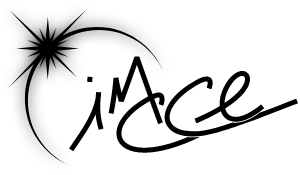
\includegraphics[width=.5\textwidth]{logo-imcce}\\
        \vspace{0.5em}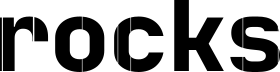
\includegraphics[width=.5\textwidth]{logo-rocks}
      \end{column}
      %      
      \begin{column}{.7\textwidth}
        \small
        \vspace{3cm}
        \textbf{B.~Carry}$^1$ \&
        \textbf{M.~Mahlke}$^2$\\
        \footnotesize{$^1$Lagrange, Observatoire de la C{\^o}te d'Azur, Nice}\\
        \footnotesize{$^1$Institut d'Astrophysique Spatiale, Orsay}
      \end{column}
    \end{columns}

  \end{center}

\end{frame}
%%%%%%%----  END  ---- Title frame ----%%%%%%
         %-Ok
  %\section{Why shared resources?}


%%%%%%%---- BEGIN ----  ----%%%%%%
\begin{frame}
  \frametitle{A typical research project}

  \begin{columns}[T]

    \begin{column}{.4\textwidth}
      \begin{overlayarea}{\textwidth}{\textheight}
        \only<1>{\hspace{0.05\hsize}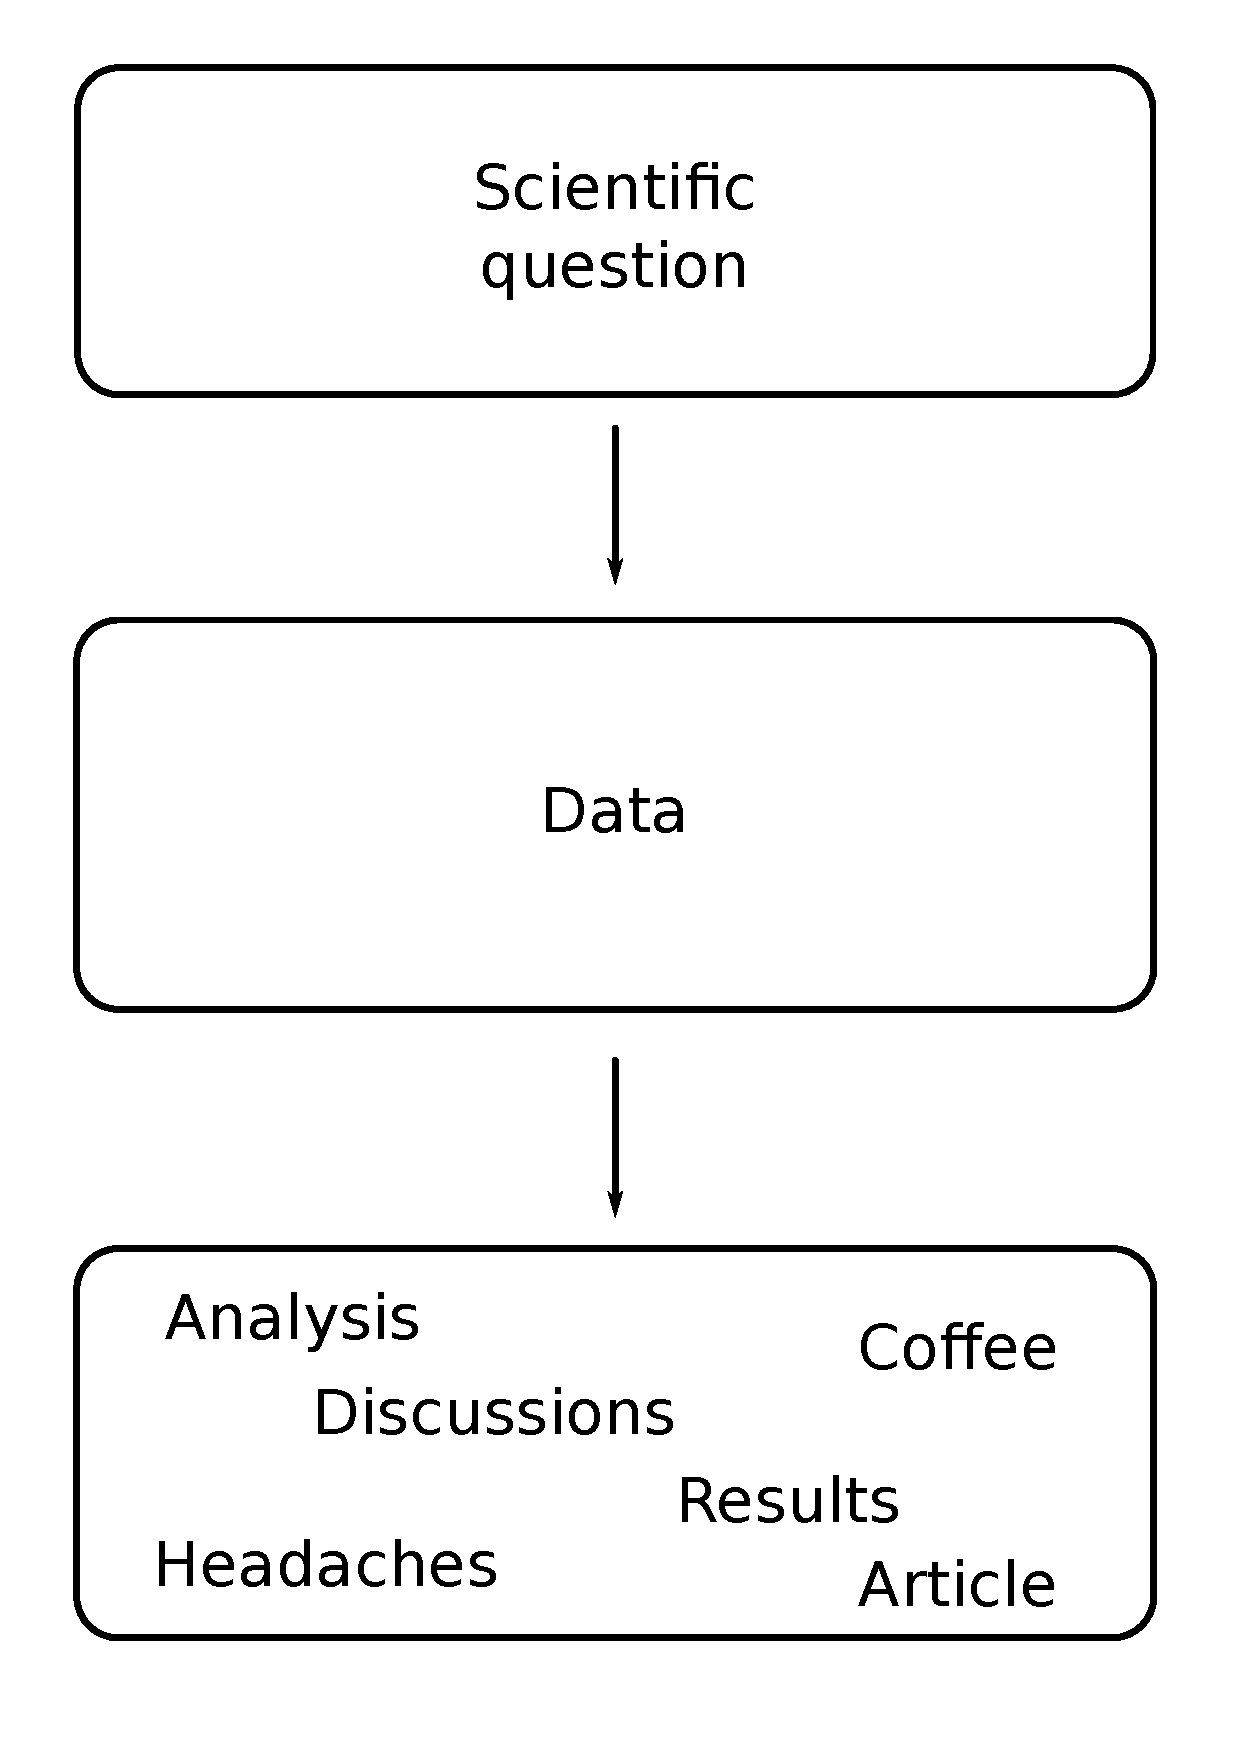
\includegraphics[width=0.9\hsize]{sci_project_1}}
        \only<2>{\hspace{0.05\hsize}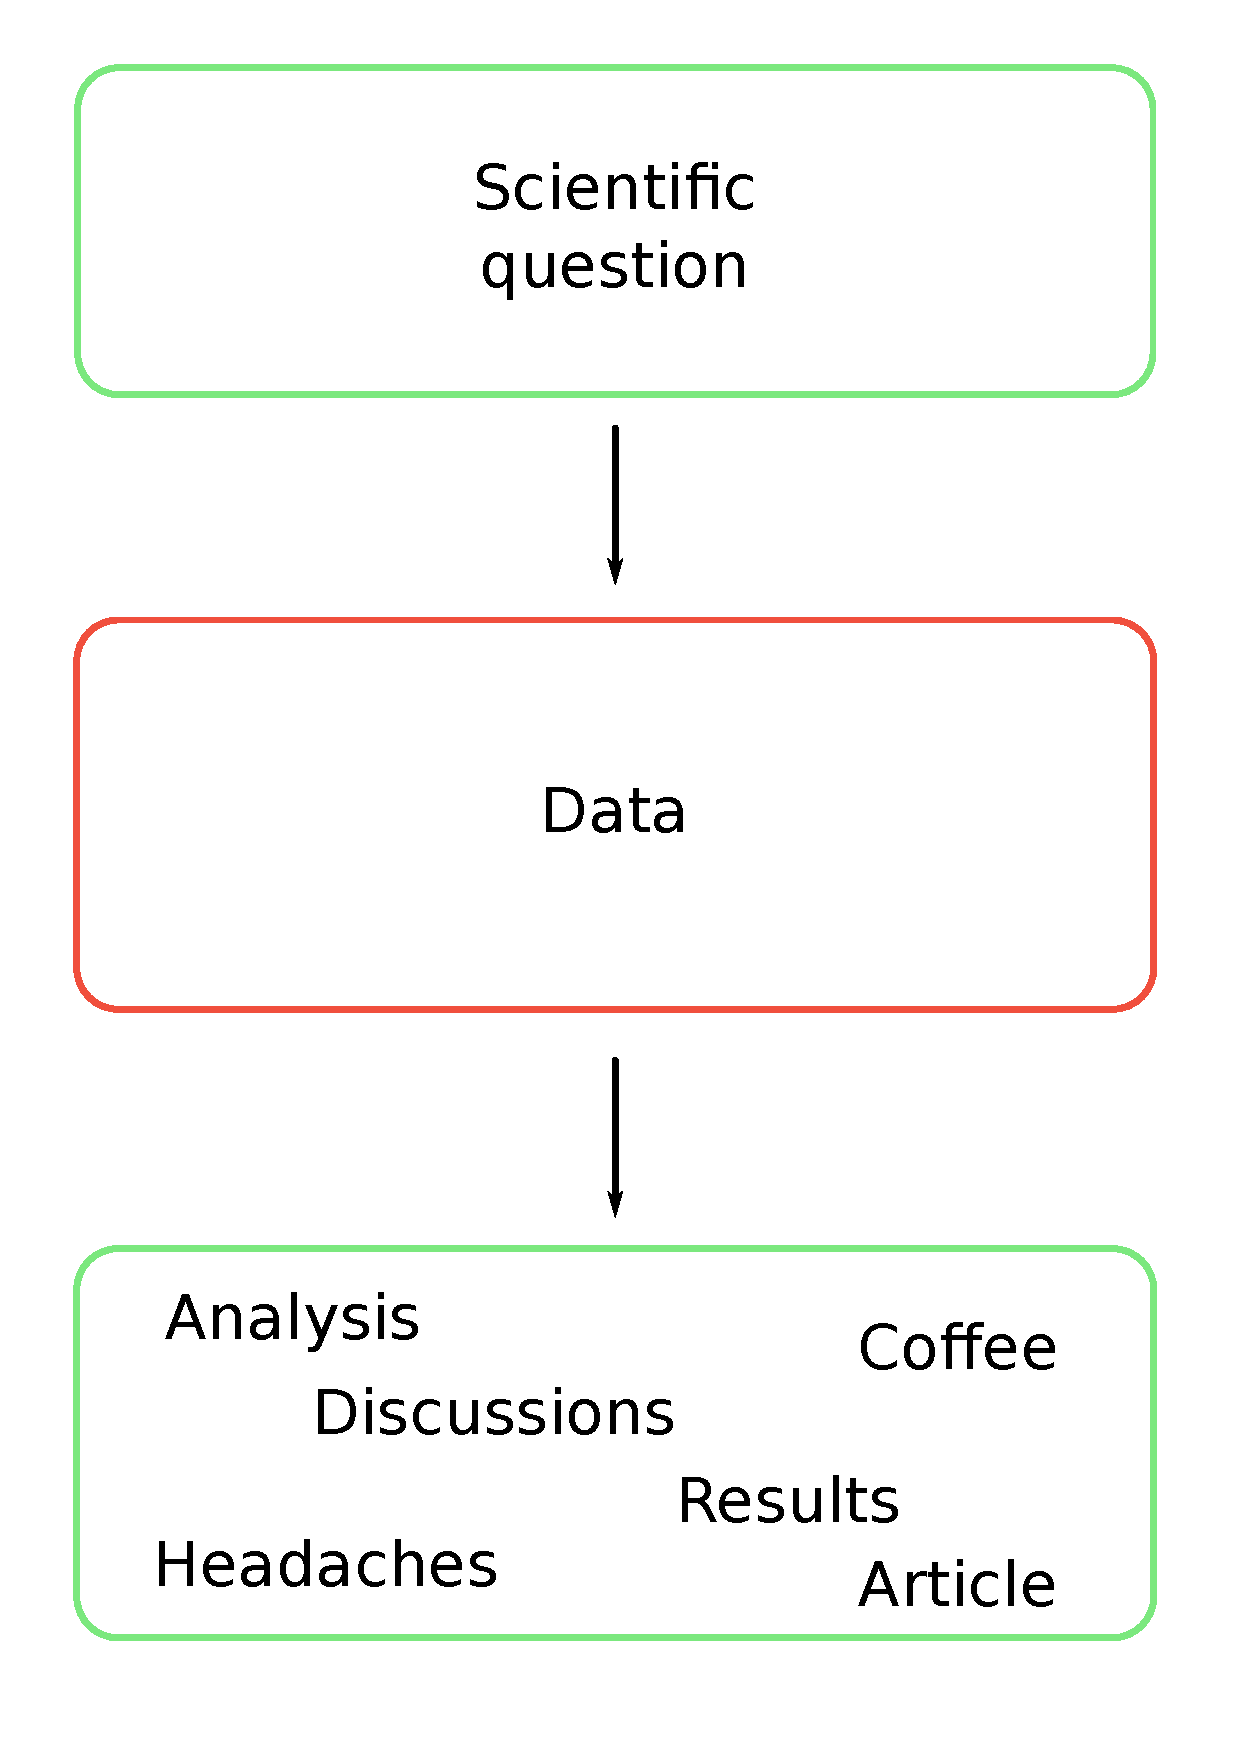
\includegraphics[width=0.9\hsize]{sci_project_2}}
      \end{overlayarea}
    \end{column}


    \begin{column}{.6\textwidth}
      \begin{overlayarea}{\textwidth}{\textheight}
        \begin{onlyenv}<2>

          \vspace{1em}
          \textbf{\bf Repetitive (and tedious) tasks!}\\
          \vspace{1em}
          \begin{itemize}[<.->]
            \item \emph{\bf Planning and conduction of observations}
              \begin{itemize}[<.->]
                \item[$\circ$] Observations already exist?
                \item[$\circ$] Target/sample available? visible?
              \end{itemize}

            \vspace{0.5em}
            \item \emph{\bf Gathering ancillary data for the analysis}
              \begin{itemize}[<.->]
                \item[$\circ$] Complementary information \src{diameter, fall/find, ...}
                \item[$\circ$] Context for research \src{another population}
              \end{itemize}

            \vspace{0.5em}
            \item \emph{\bf Repetitive low-level analysis}
              \begin{itemize}[<.->]
                \item[$\circ$] Spectral classification
                \item[$\circ$] Cross-matches \& merges
              \end{itemize}

          \end{itemize}
        \end{onlyenv}
      \end{overlayarea}
    \end{column}
  
  \end{columns}

\end{frame}
%%%%%%%----  END  ----  ----%%%%%%



%%%%%%%---- BEGIN ----  ----%%%%%%
\begin{frame}
  \frametitle{Shared resources save community time}

  \begin{itemize}[<.->]
    \item \emph{\bf Tedious tasks? Share the load!}
      \begin{itemize}[<.->]
        \item[$\circ$] Many agencies have the mission to support the community
        \item[] \src{ESO/ESA/NASA, JPL/MPC/IMCCE, ...}
        \item[$\circ$] The expertize is in the community $\rightarrow$ individual initiatives
        \item[] \src{SSHADE, Meteoretical Bulletin, SMASS}
        \item[$\blacktriangleright$] More time for your research
      \end{itemize}
  
    \vspace{0.5em}
  \item \emph{\bf Tedious tasks? Automatize them!}
      \begin{itemize}[<.->]
        \item[$\circ$] Click, click, click... copy-paste, click...
        \item[$\circ$] Or code some processes to work for you
        \item[$\blacktriangleright$] Virtual Observatory \& Community librairies
      \end{itemize}
  
    \vspace{0.5em}
    \item \emph{\bf Community services are less prone to errors!}
      \begin{itemize}[<.->]
        \item[$\circ$] One user $\rightarrow$ one $\alpha$-, $\beta$-tester, user...
        \item[$\circ$] Many users $\rightarrow$ bug reports! and community solutions \& patches!
        \item[$\blacktriangleright$] Robustness of analysis $\rightarrow$ results
      \end{itemize}

  \end{itemize}
  
\end{frame}
%%%%%%%----  END  ----  ----%%%%%%




           %-Ok
  \section{Examples}

\subsection{Pointing a telescope}
%%%%%%%---- BEGIN ----  ----%%%%%%
\begin{frame}
  \frametitle{Pointing a telescope}

  \begin{overlayarea}{\textwidth}{0.15\textheight}
    \vspace{-0.5em}
    \begin{exampleblock}{Example}
      Where do I point the telescope from the name of a target?
    \end{exampleblock}
  \end{overlayarea}

  \begin{overlayarea}{\textwidth}{0.8\textheight}
    \begin{onlyenv}<2>
      \begin{block}{Answer: CDS, IMCCE Miriade, JPL SSD, MPC, Lowell AstEph}
        \hspace{.10\hsize}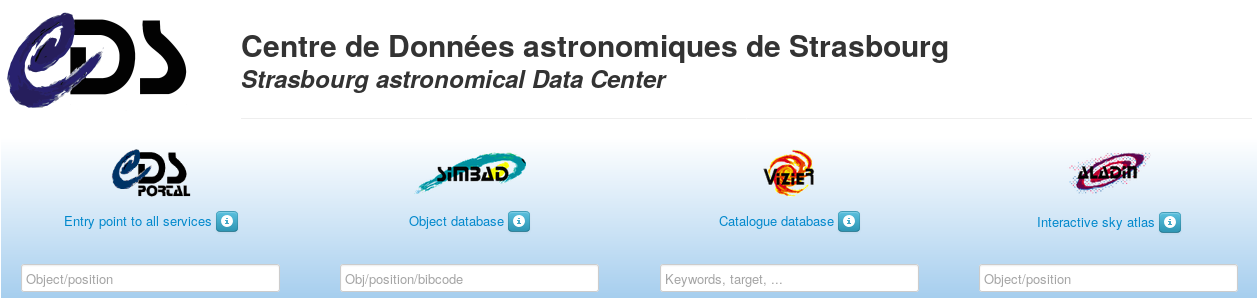
\includegraphics[width=.45\hsize]{portal-cds}\\
        \hspace{.35\hsize}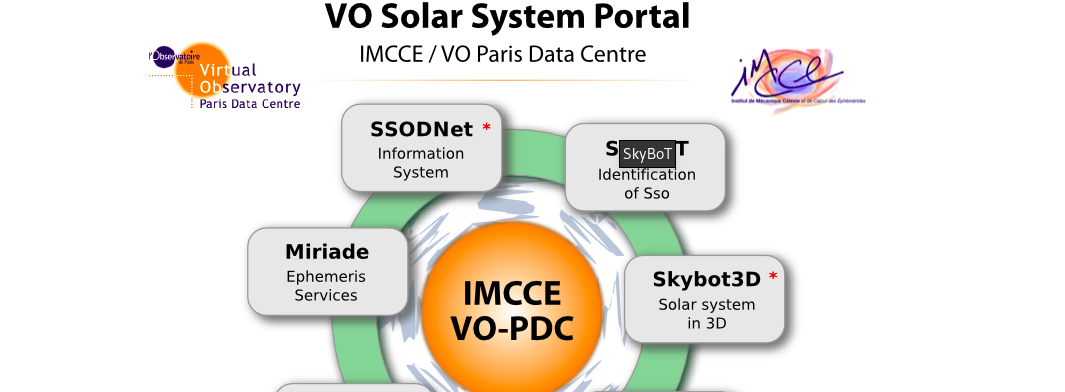
\includegraphics[width=.45\hsize]{portal-imcce}
      \end{block}
    \end{onlyenv}
  \end{overlayarea}

\end{frame}
%%%%%%%----  END  ----  ----%%%%%%


\subsection{Visibility of targets}
%%%%%%%---- BEGIN ----  ----%%%%%%
\begin{frame}
  \frametitle{Visibility of targets}

  \begin{overlayarea}{\textwidth}{0.15\textheight}
    \vspace{-0.5em}
    \begin{exampleblock}{Example}
      Can I observe asteroids Raymond, Delsanti, 7561 and 10281? And M31 and M67?
    \end{exampleblock}
  \end{overlayarea}

  \begin{overlayarea}{\textwidth}{0.8\textheight}
    \begin{onlyenv}<2>
      \begin{block}{Answer: IMCCE ViSiON, Lowell AstObs, airmass.org}
        \hspace{.25\textwidth}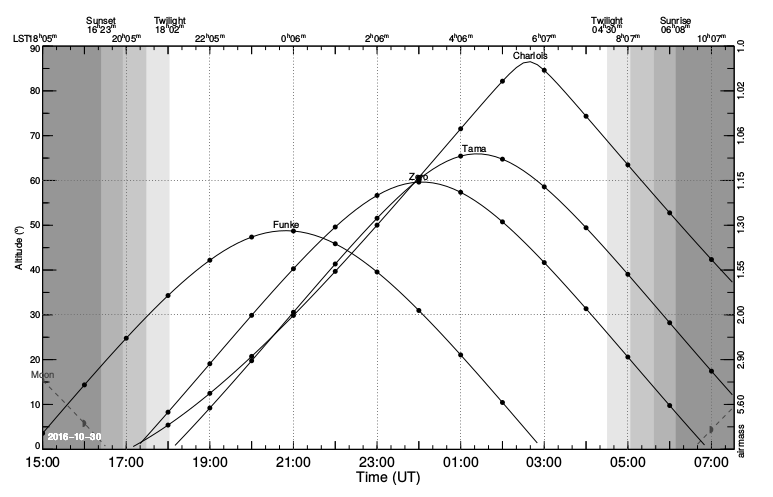
\includegraphics[width=.5\textwidth]{vision}
      \end{block}
    \end{onlyenv}
  \end{overlayarea}
% https://ssp.imcce.fr/webservices/miriade/api/vision.php?-name=a:Raymond,a:Patrickmichel,a:Libourel,a:Delsanti,u:M67,u:M31&-nbd=1&-step=1&-observer=010&-ep=2024-02-06&-from=Demo&-mime=pdf
\end{frame}
%%%%%%%----  END  ----  ----%%%%%%

\subsection{Accessing data}
%%%%%%%---- BEGIN ----  ----%%%%%%
\begin{frame}
  \frametitle{Accessing data}

  \begin{overlayarea}{\textwidth}{0.15\textheight}
    \vspace{-0.5em}
    \begin{exampleblock}{Example}
      What is the taxonomy of Vernazza? the diameter of Groussin?
    \end{exampleblock}
  \end{overlayarea}

  \begin{overlayarea}{\textwidth}{0.8\textheight}
    \begin{onlyenv}<2>
      \begin{block}{Answer: IMCCE SsODNet, JPL sbdb, OCA MP3C, Lowell AstInfo, SiMDA}
        \hspace{.05\hsize}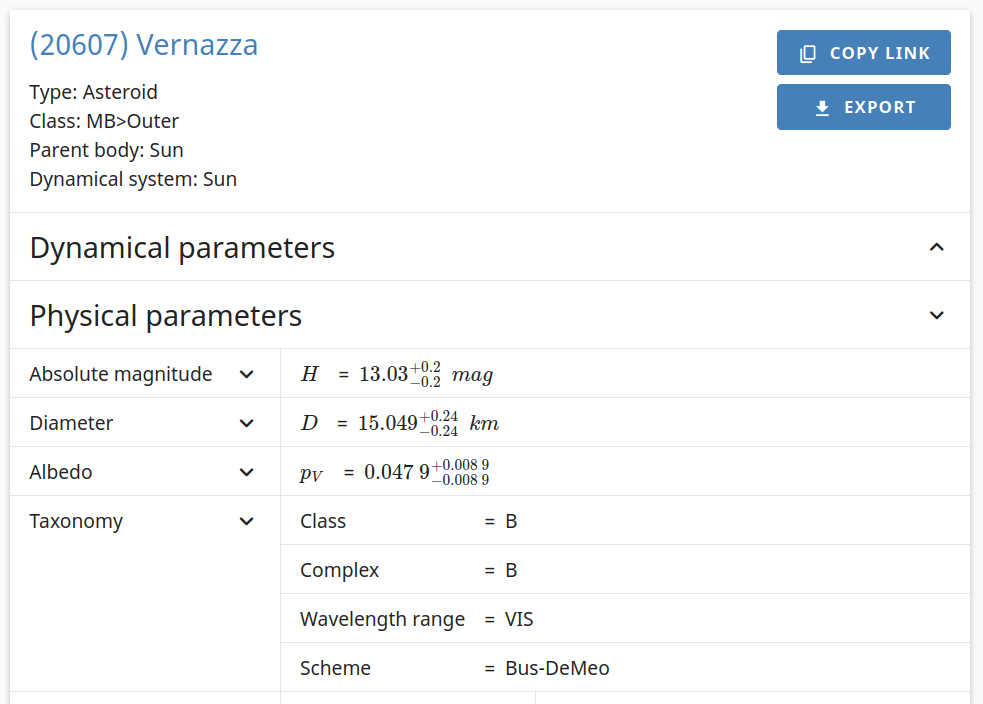
\includegraphics[width=.4\hsize]{ssodnet-vernazza}
        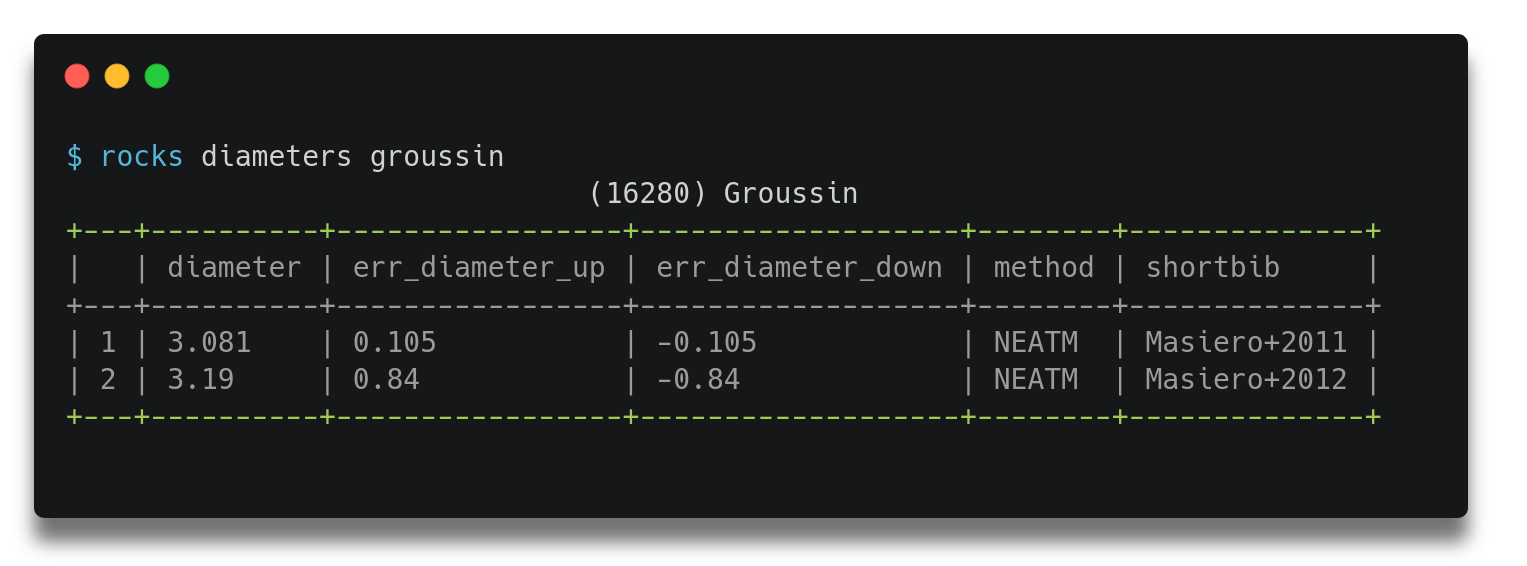
\includegraphics[width=.5\hsize]{ssodnet-groussin}
      \end{block}
    \end{onlyenv}
  \end{overlayarea}

\end{frame}
%%%%%%%----  END  ----  ----%%%%%%
       %-Ok
  %\section{What is the Virtual Observatory?}

%%%%%%%---- BEGIN ----  ----%%%%%%
\begin{frame}
  \frametitle{The Virtual Observatory}

  \begin{itemize}[<+->]
    \item \emph{Is a suite of services and tools}
      \begin{itemize}[<.->]
        \item[$\circ$] \textbf{Provider:} archives, catalogs, on-line codes
        \item[$\circ$] \textbf{Client:} GUI, analysis tools
        \item[$\circ$] \url{http://ivoa.net/astronomers/applications.html}
      \end{itemize}

    \vspace{1em}
    \item \emph{Is a suite of standards}
      \begin{itemize}[<.->]
        \item[$\circ$] Common interface (e.g., I/O VOTable =xml)
        \item[$\circ$] Registries, semantic
        \item[$\circ$] \url{http://ivoa.net/deployers/}
      \end{itemize}

    \vspace{1em}
    \item \emph{Is \textbf{not} a master software}

    \vspace{1em}
    \item \emph{Is made by us, and for us}
      \begin{itemize}[<.->]
        \item[$\circ$] Powerful libraries and tools
        \item[$\circ$] Good practice to release data/codes
      \end{itemize}

  \end{itemize}

\end{frame}
%%%%%%%----  END  ----  ----%%%%%%


            %-Ok
  %\section{My favorites}


%%%%%%%---- BEGIN ----  ----%%%%%%
\begin{frame}
  \frametitle{Some amazing services}

  \begin{itemize}
    \item \emph{CDS: SIMBAD, VizieR, and Aladin}
      \begin{itemize}[<.->]
        \item \textbf{THE} place for catalogs
        \item Multi-function GUI \& Web API
      \end{itemize}

    \vspace{0.5em}
    \item \emph{IMCCE: SSO Portal}
      \begin{itemize}[<.->]
        \item Online computation of ephemerides: \texttt{Miriade} \& \texttt{SkyBoT}
        \item Observation planning: \texttt{ViSiON}
        \item Spectral modeling: \texttt{M4Ast}
      \end{itemize}

    \vspace{0.5em}
    \item \emph{SVO: VOSA, Filter profiles, SED models}
      \begin{itemize}[<.->]
        \item Magnitude-Flux-Energy conversion
        \item Collection of photometry 
        \item SED fitting
      \end{itemize}

    \vspace{0.5em}
    \item \emph{Miscellaneous but great!}
      \begin{itemize}[<.->]
        \item SSOIS: SSO image search
        \item ESA-Sky: explore ESA archive
        \item VOStat: VO interface to R
      \end{itemize}
  \end{itemize}

\end{frame}
%%%%%%%----  END  ----  ----%%%%%%
          %-

%
\end{document}
